\section{Hovedrutine}
I dette afsnit beskrives programmets hovedloop i grove træk, for at give en forståelse af BMS's funktionalitet. Systemet har en del funktioner som skal gennemføres for at opnå alle ønskede funktionaliteter og beskyttelser. Fælles for både den diskrete og den integrerede version af BMS'en, er at hovedrutinen, eller specifikt, de enkelte funktioners rækkefølge og funktionalitet, hovedsageligt er den samme. Derfor vil de ikke forklares hver for sig, hvis den eneste forskel f.eks. er at en I2C kommando på IC versionen erstattes med et GPIO signal på den diskrete. Er der markante ændringer forklares de i de to seperate underafsnit. \\

\begin{figure}[h]
	\centering
	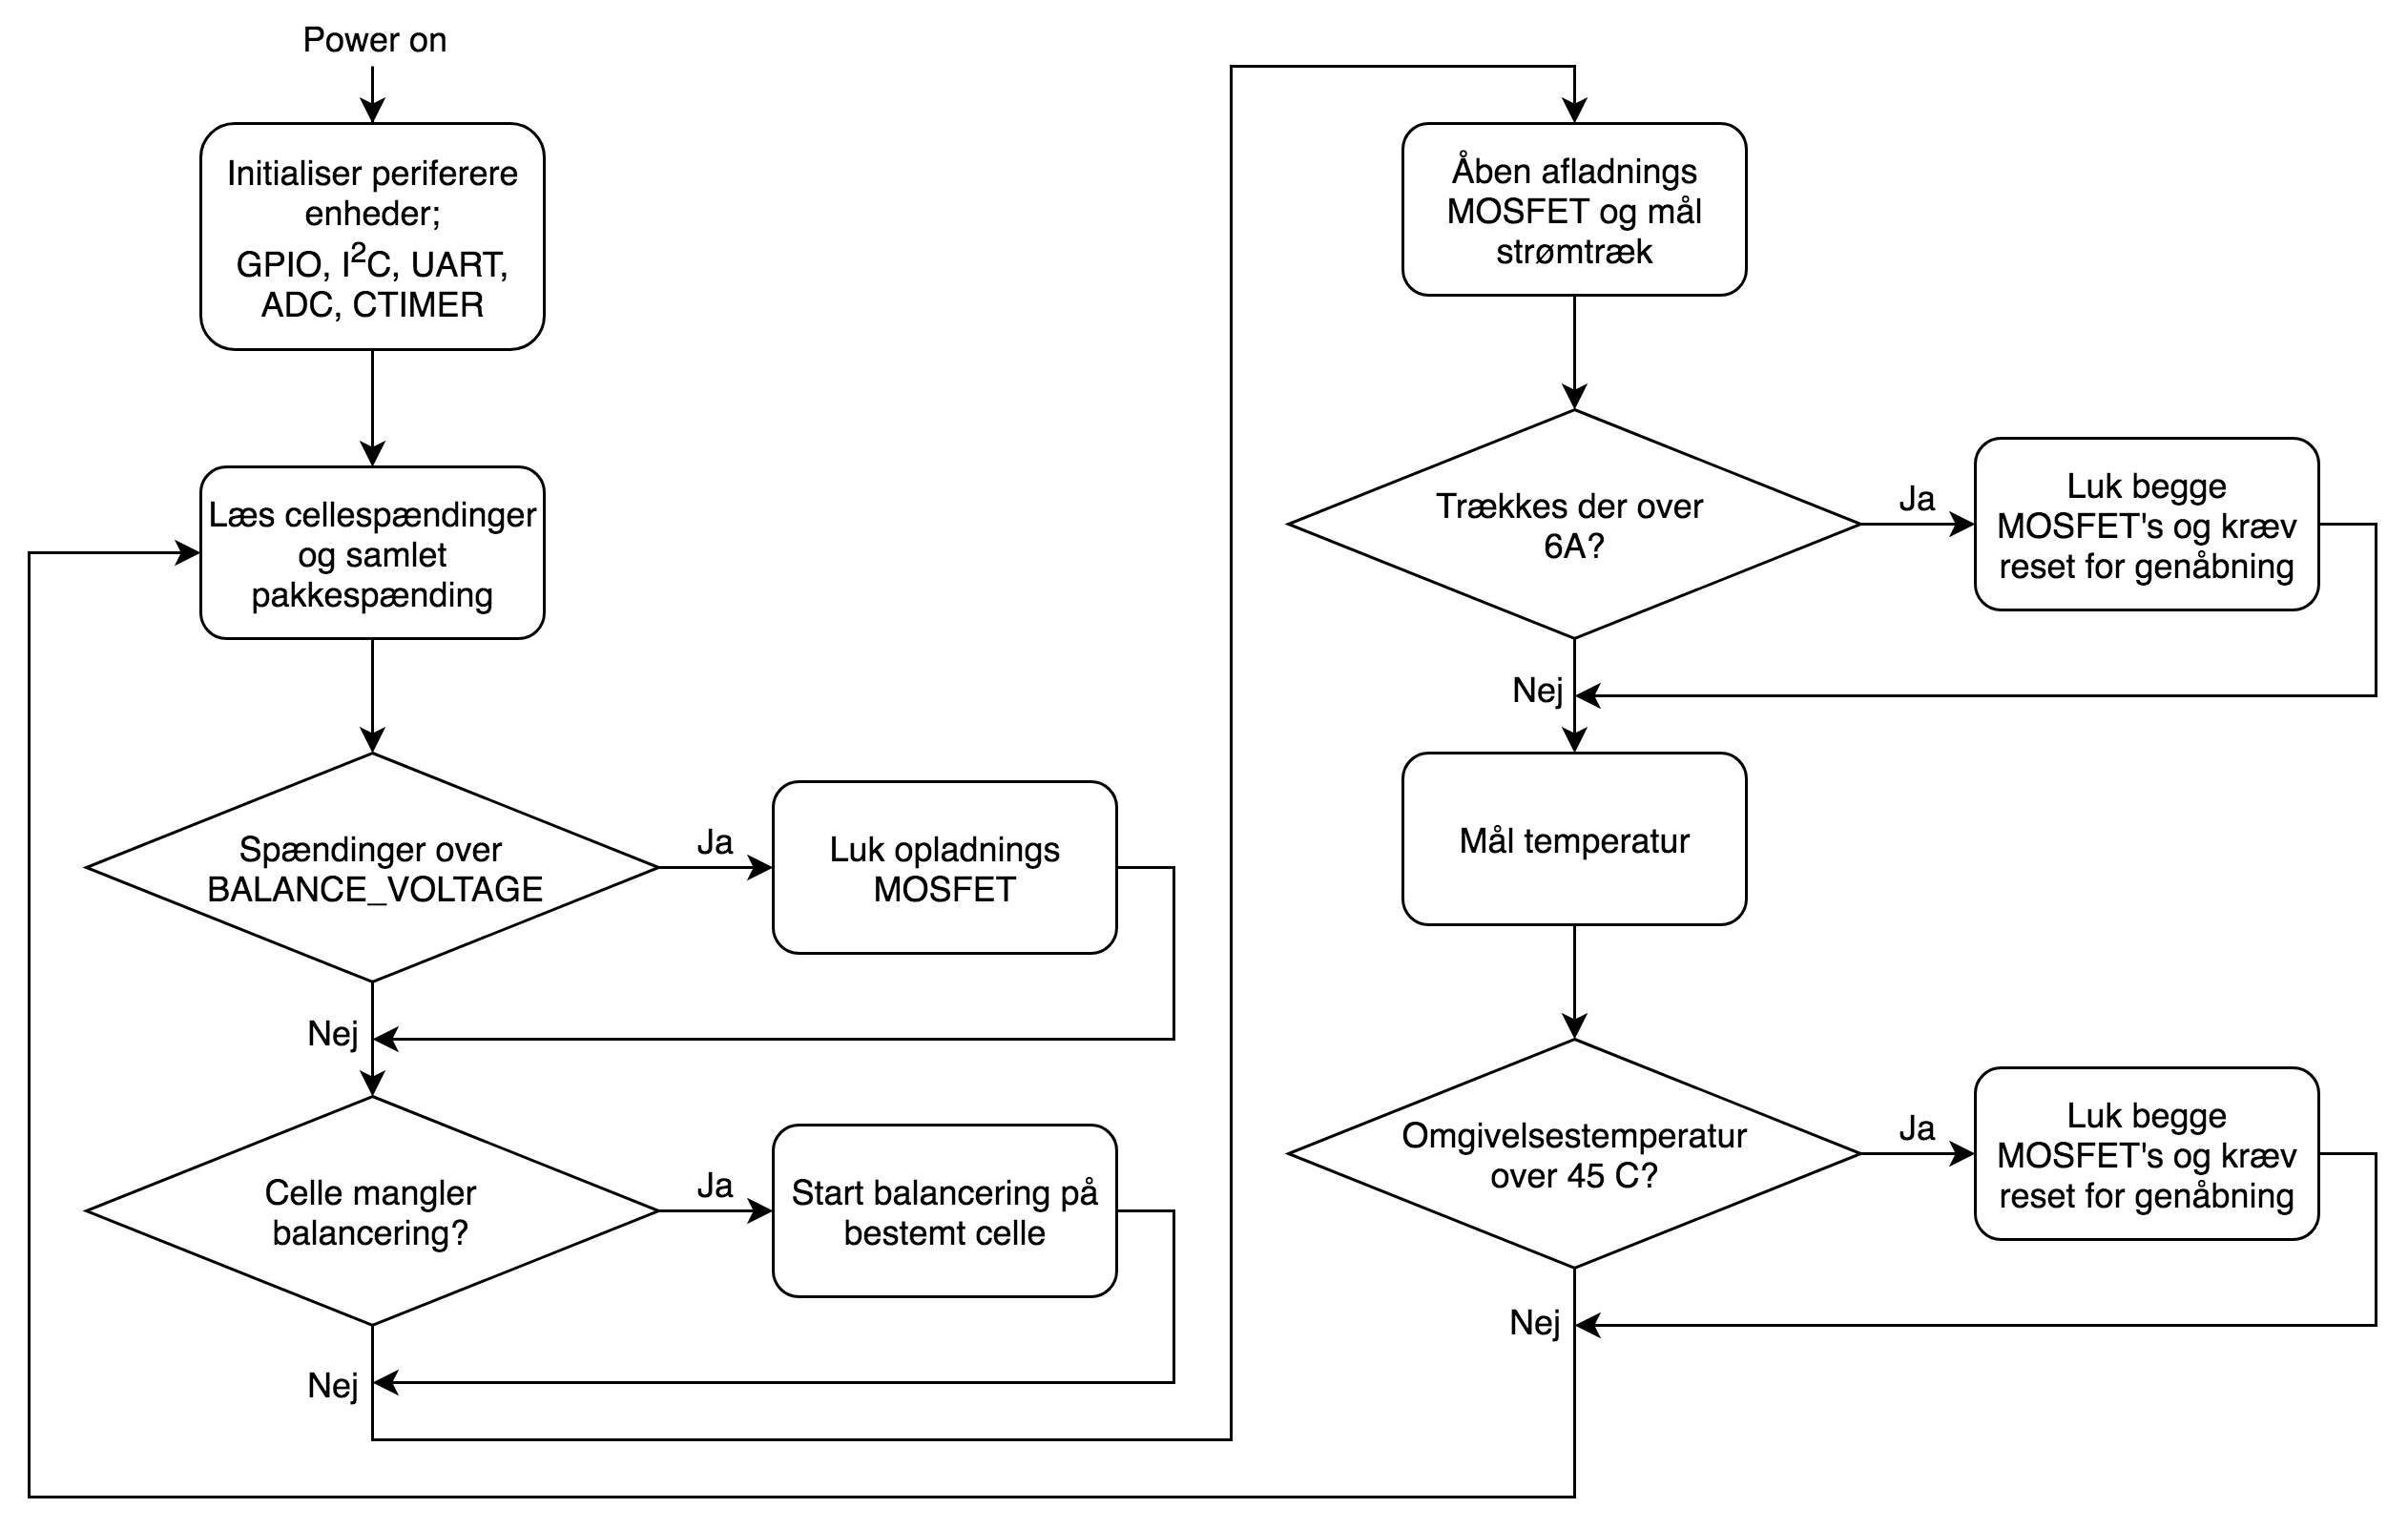
\includegraphics[width=15cm]{billeder/main_loop_bms_functions.png}
	\caption{Simplificeret flowchart over main loop (fokus på BMS funktionerne)}
	\label{fig:main_loop}
\end{figure}

På figur \ref{fig:main_loop} ses flowchartet for hovedrutinen. Der startes med at hente alle de tilgængelige informationer om batteripakken. Her udregnes de brugbare informationer som samlet pakkespænding, procent baseret på spænding, strømtræk, tilbageværende kapacitet baseret på strømtræk (coulomb counting) og temperatur. Mere om kapacitet og procentudregning i afsnit \ref{afs:SOC_realization}. Disse værdier bruges til balancerings- og sikkerhedsfunktionerne på BMS'en. \\

Først tjekkes balanceringen. Her sammenlignes cellespændingerne med de valgte spændings \space "lofte" \space og de andre cellespændinger. Er alle celler lig med \verb|BALANCE_VOLTAGE|, stoppes opladningen og der gives besked til brugeren. Hvis ikke, tjekkes de næste celler. Tages der udgangspunkt i celle 1 lyder rækkefølgen af checks som følger. Hvis celle 1 er over \verb|BALANCE_VOLTAGE| (som er den valgte spænding cellerne skal balanceres til), og samtidig er større end både celle 2, 3 og 4, skal denne balanceres ned først. Balanceringen stoppes når spændingen når ned på, eller under, celle 2, 3 og 4's spændinger. Det samme gøres for de resterende celler. Er ingen af disse kriterier opfyldt, tillades opladning på fuldt blus da cellerne er ønsket kapacitet.\\

Dernæst kommer beskyttelsesfunktionerne. Her tages der udgangspunkt i strømmålingen, og er denne over $6\ampere$ lukkes der for begge MOSFET's, og der gives besked til brugeren om, at et reset er nødvendigt for at kunne fortsætte. Til sidst i rutinen laves en temperaturmåling. \\

\subsection{Diskret BMS}
Den diskrete BMS bruger en del ADC'ere og GPIO pins til styring af alle funktionaliteterne, så derfor sættes disse op først. UART'en initialiseres også og en statup besked sendes. Derefter skal alle relevante spændinger sættes for at styre BMS'en som ønsket og er forklaret nærmere i afsnit \ref{afs:ADC} og \ref{afs:PWM}.

\subsection{Integreret BMS}
I den integrerede BMS initialiseres systemet med at klargøre alle protokoller. Som i den diskrete, sendes en startup-meddelelse på UART porten. Efter initialisation kører de fleste rutiner over I2C. BQ76920 skal initialiseres med de ønskede indstillinger i register $0x04$ og $0x05$. Her sættes bit 4 i $0x04$ for at aktivere ADC'en, og bit 6 i $0x05$, for at aktivere strømmåleren i kredsen. Register $0x0B$ skal overskrives med $0x19$ under opstart ifølge databladet.\footnote{\url{http://www.ti.com/lit/ds/symlink/bq76920.pdf} side 41} \\

Derudover er der 3 "PROTECT" \space registre der skal indstilles. I PROTECT1 ($0x06$) sættes bit 7 for at fordoble RSNS værdien. Dette gøres for at kunne måle op til (og faktisk over) $6\ampere$ med en shunt modstand på $0.01\ohm$. Bit 0-2 sættes til 1 for at tillade maksimum strøm ved kortslutning da det alligevel er noget microen står for. Det samme gøres i PROTECT2($0x07$) (bit 0-3) for at tillade maksimum strømtræk da dette også er begrænset med microen. PROTECT3($0x08$) ændres ikke, og der køres derfor med default værdier. Alle disse registre sættes i \verb|BMS_Init()|.

